\documentclass[12pt, a4paper]{article}

% Packages
\usepackage[utf8]{inputenc}
\usepackage{graphicx}
\usepackage{geometry}
\usepackage{booktabs} % For professional tables
\usepackage{float}    % For precise image placement [H]
\usepackage{hyperref}
\usepackage{caption}
\usepackage{subcaption}
\usepackage{amsmath}
\usepackage{listings}
\usepackage{xcolor}
\usepackage{array}

% Image Path Configuration
\graphicspath{ {./report_images/} }

% Margins
\geometry{
 a4paper,
 total={170mm,257mm},
 left=25mm,
 top=25mm,
}

% Title Data
\title{\textbf{Comparative Analysis of Machine Learning Models for Spotify Genre Classification}\\
\large Term Project (Data Science II)}
\author{
\textbf{Group 8} \\
Anvita Yerramsetty \\
Austin Bell \\
Carter Prince \\
Robera Abajobir \\
Sanghyun An \\
Tyler Varma
}
\date{November 25, 2025}

\begin{document}

\maketitle

\begin{abstract}
This study evaluates the performance of six distinct machine learning algorithms in predicting the musical genre of Spotify tracks based on tabular audio features and metadata. Using a dataset of approximately 47,000 songs across 24 genres, a preprocessing pipeline was implemented to address class imbalance and feature scaling. The models evaluated include Logistic Regression, K-Nearest Neighbors, Gaussian Naive Bayes, Random Forest, XGBoost, and a Multilayer Perceptron. Results indicate that ensemble tree-based methods yield the highest predictive performance, with XGBoost achieving an accuracy of 54.37\%. This performance notably exceeds the random baseline of 4.1\%, suggesting that while audio summary features contain predictive signal, the complexity of genre boundaries limits the effectiveness of tabular classification methods.
\end{abstract}

\tableofcontents
\newpage

\section{Problem Statement}
Music genre classification is a fundamental task in Music Information Retrieval (MIR), essential for the functionality of streaming platforms such as Spotify and Apple Music. Accurate classification supports recommendation systems, playlist generation, and user personalization.

The classification task presents challenges due to the subjective nature of musical genres and the difficulty of representing temporal audio signals as static numerical features. The objective of this study is to develop a multi-class classification model capable of predicting one of 24 distinct genres given a set of 14 high-level audio features (e.g., danceability, energy, tempo) and metadata.

\section{Collection and Description of Datasets}
The dataset utilized is \texttt{SpotifyFeatures.csv}, containing tracks retrieved via the Spotify Web API.

\subsection{Dataset Characteristics}
\begin{itemize}
    \item \textbf{Total Samples:} 46,985 (post-cleaning).
    \item \textbf{Classes:} 24 unique genres, including \textit{Alternative, Anime, Classical, Country, Electronic, Hip-Hop, Jazz, Pop, Rap, Reggaeton, Rock,} and others.
    \item \textbf{Input Features:} 14 total features.
    \begin{itemize}
        \item \textbf{Audio Metrics (Continuous):} \texttt{acousticness}, \texttt{danceability}, \texttt{energy}, \texttt{instrumentalness}, \texttt{liveness}, \texttt{loudness}, \texttt{speechiness}, \texttt{tempo}, \texttt{valence}.
        \item \textbf{Metadata (Continuous):} \texttt{popularity}, \texttt{duration\_ms}.
        \item \textbf{Musical Structure (Categorical):} \texttt{time\_signature}, \texttt{key}, \texttt{mode}.
    \end{itemize}
\end{itemize}

\section{Data Preprocessing Techniques Applied}
A standardized preprocessing pipeline was implemented using Python to ensure data quality and consistent evaluation.

\subsection{Data Cleaning and Engineering}
Initial inspection revealed tracks associated with multiple genres. To establish a single-label classification problem, tracks with duplicate IDs across different genre labels were removed. Additionally, the genre "Rap" was merged into "Hip-Hop" due to high similarity in feature space, and "A Capella" was excluded due to insufficient sample size.

\subsection{Hybrid Balancing Strategy}
To address class imbalance, a hybrid resampling strategy was applied. Majority classes were undersampled to a maximum of 2,000 samples, while minority classes were retained in their entirety. As illustrated in Figure \ref{fig:balance}, this approach reduced bias toward dominant classes while preserving information from minority classes.

\begin{figure}[H]
    \centering
    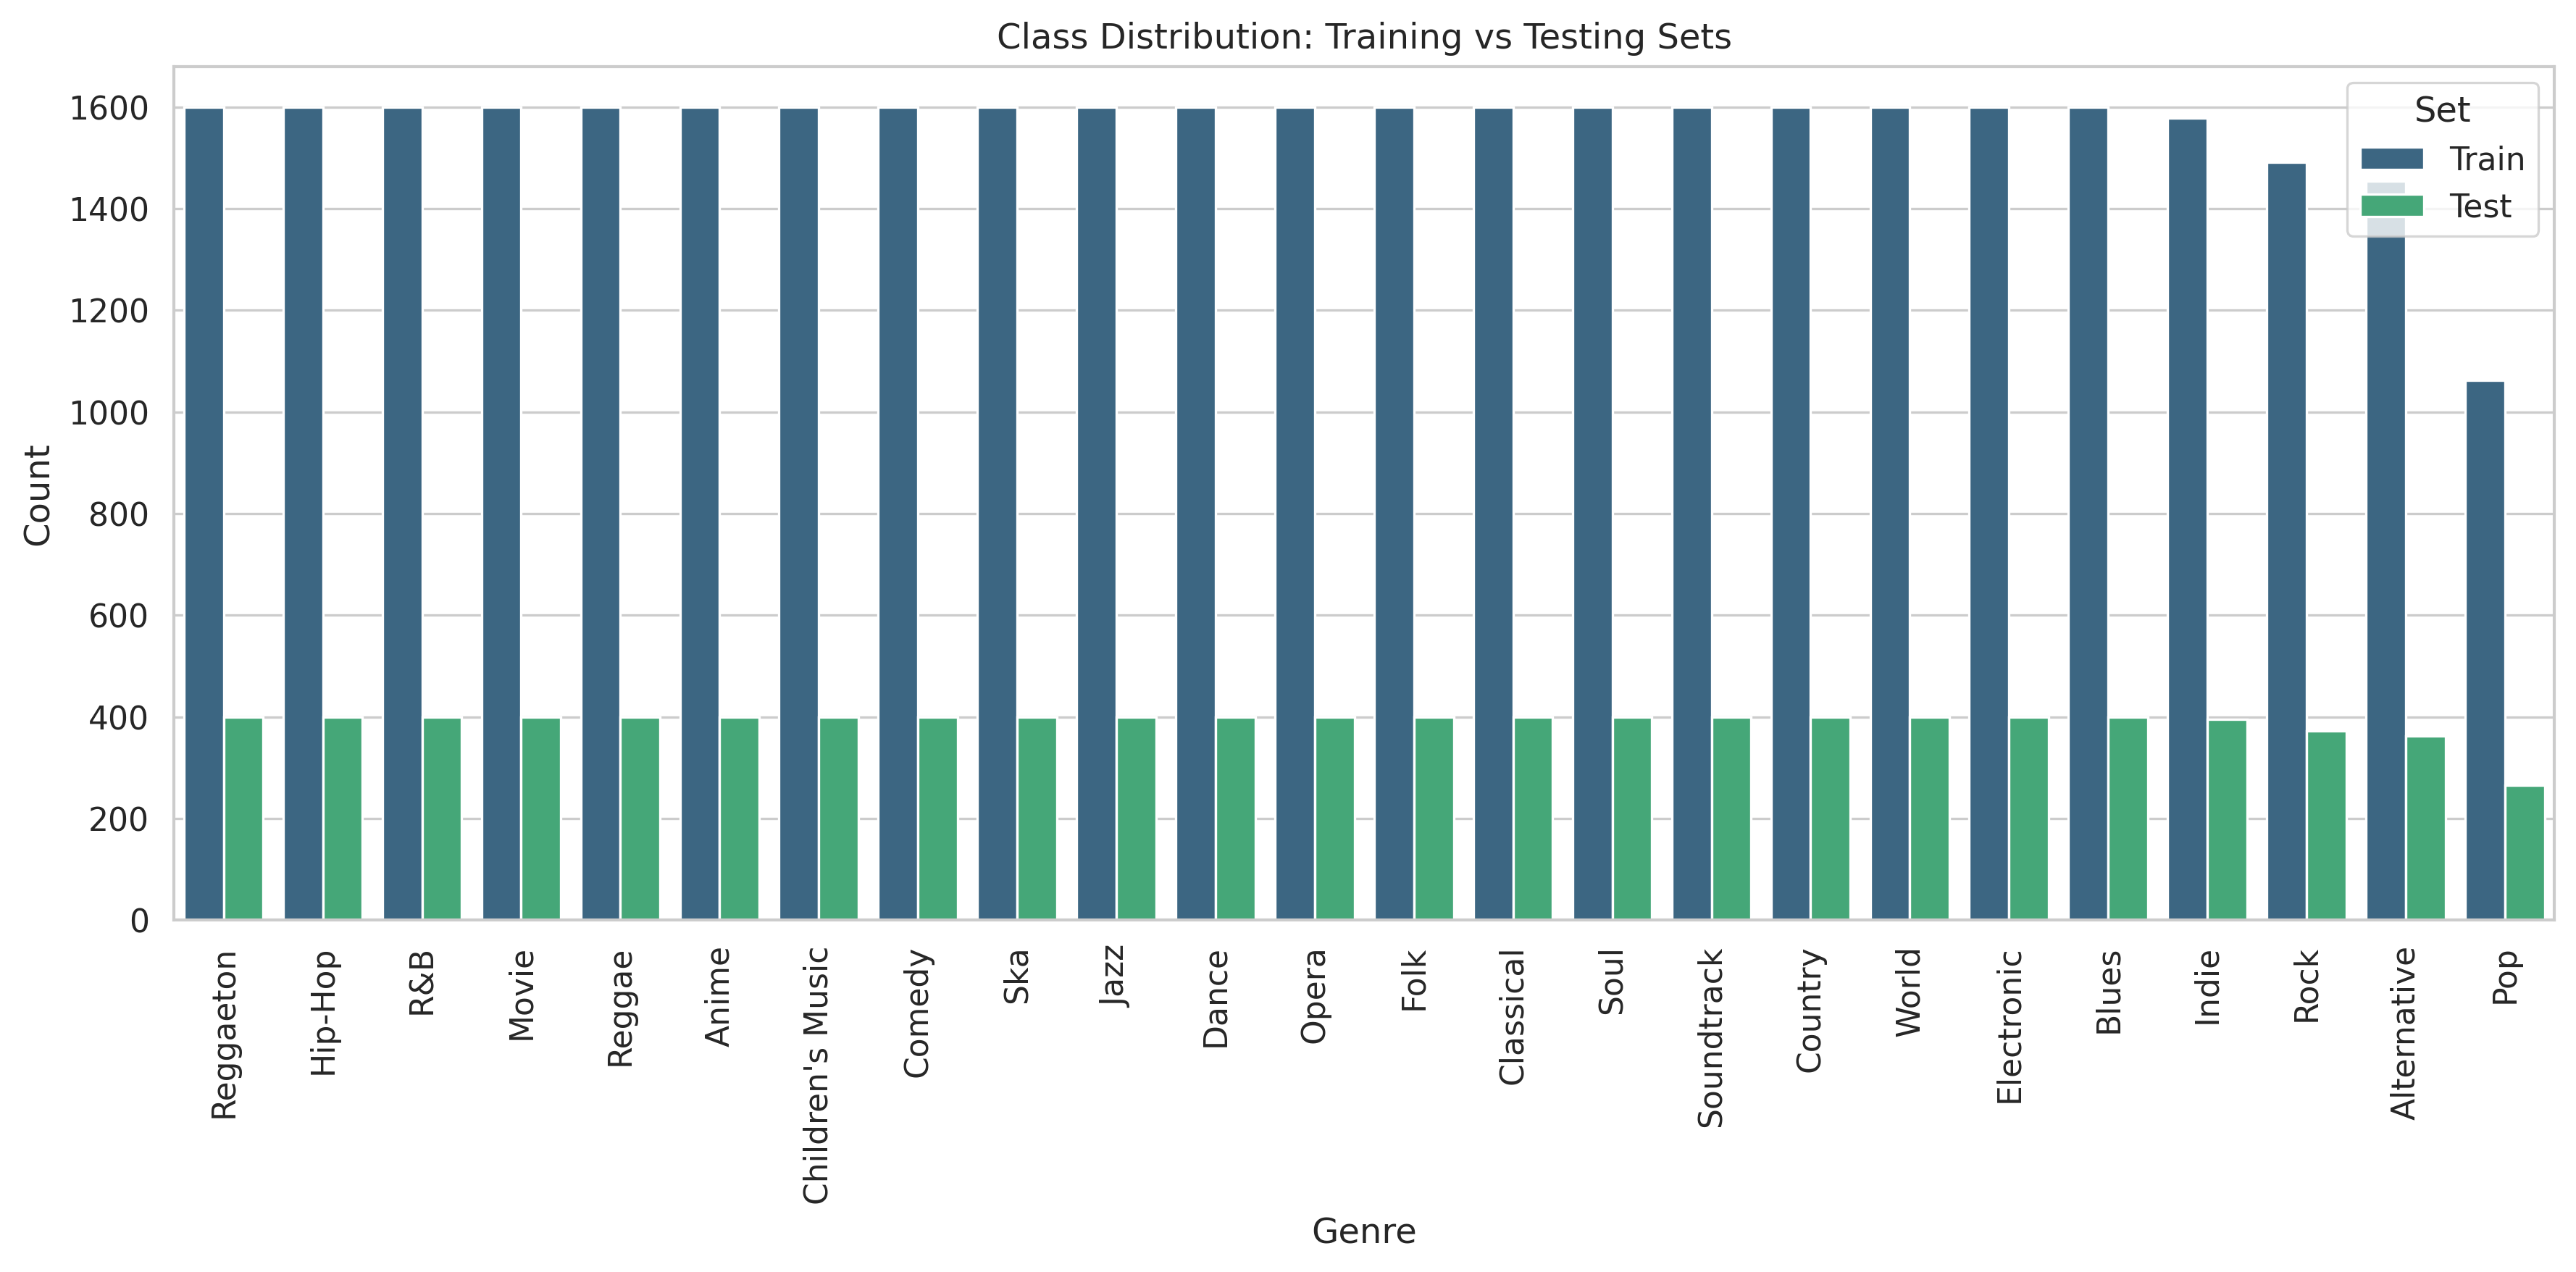
\includegraphics[width=0.9\textwidth]{fig1_class_balance.png}
    \caption{Class distribution in Training and Testing sets following hybrid balancing.}
    \label{fig:balance}
\end{figure}

\subsection{Scaling and Encoding}
\texttt{StandardScaler} (Z-score normalization) was applied to all continuous features to facilitate the convergence of gradient-based models (MLP, Logistic Regression) and the accuracy of distance-based models (KNN). Categorical features were encoded using Label Encoding.

\section{Visual Examination}
Exploratory Data Analysis (EDA) was conducted to assess feature relationships and class separability.

\subsection{Correlation Analysis}
The Pearson correlation matrix (Figure \ref{fig:corr}) indicates multicollinearity among specific audio features. A correlation coefficient of $0.82$ was observed between \texttt{energy} and \texttt{loudness}, while \texttt{acousticness} and \texttt{energy} exhibited a negative correlation of $-0.74$. These correlations suggest that models assuming feature independence, such as Naive Bayes, may experience performance degradation.

\begin{figure}[H]
    \centering
    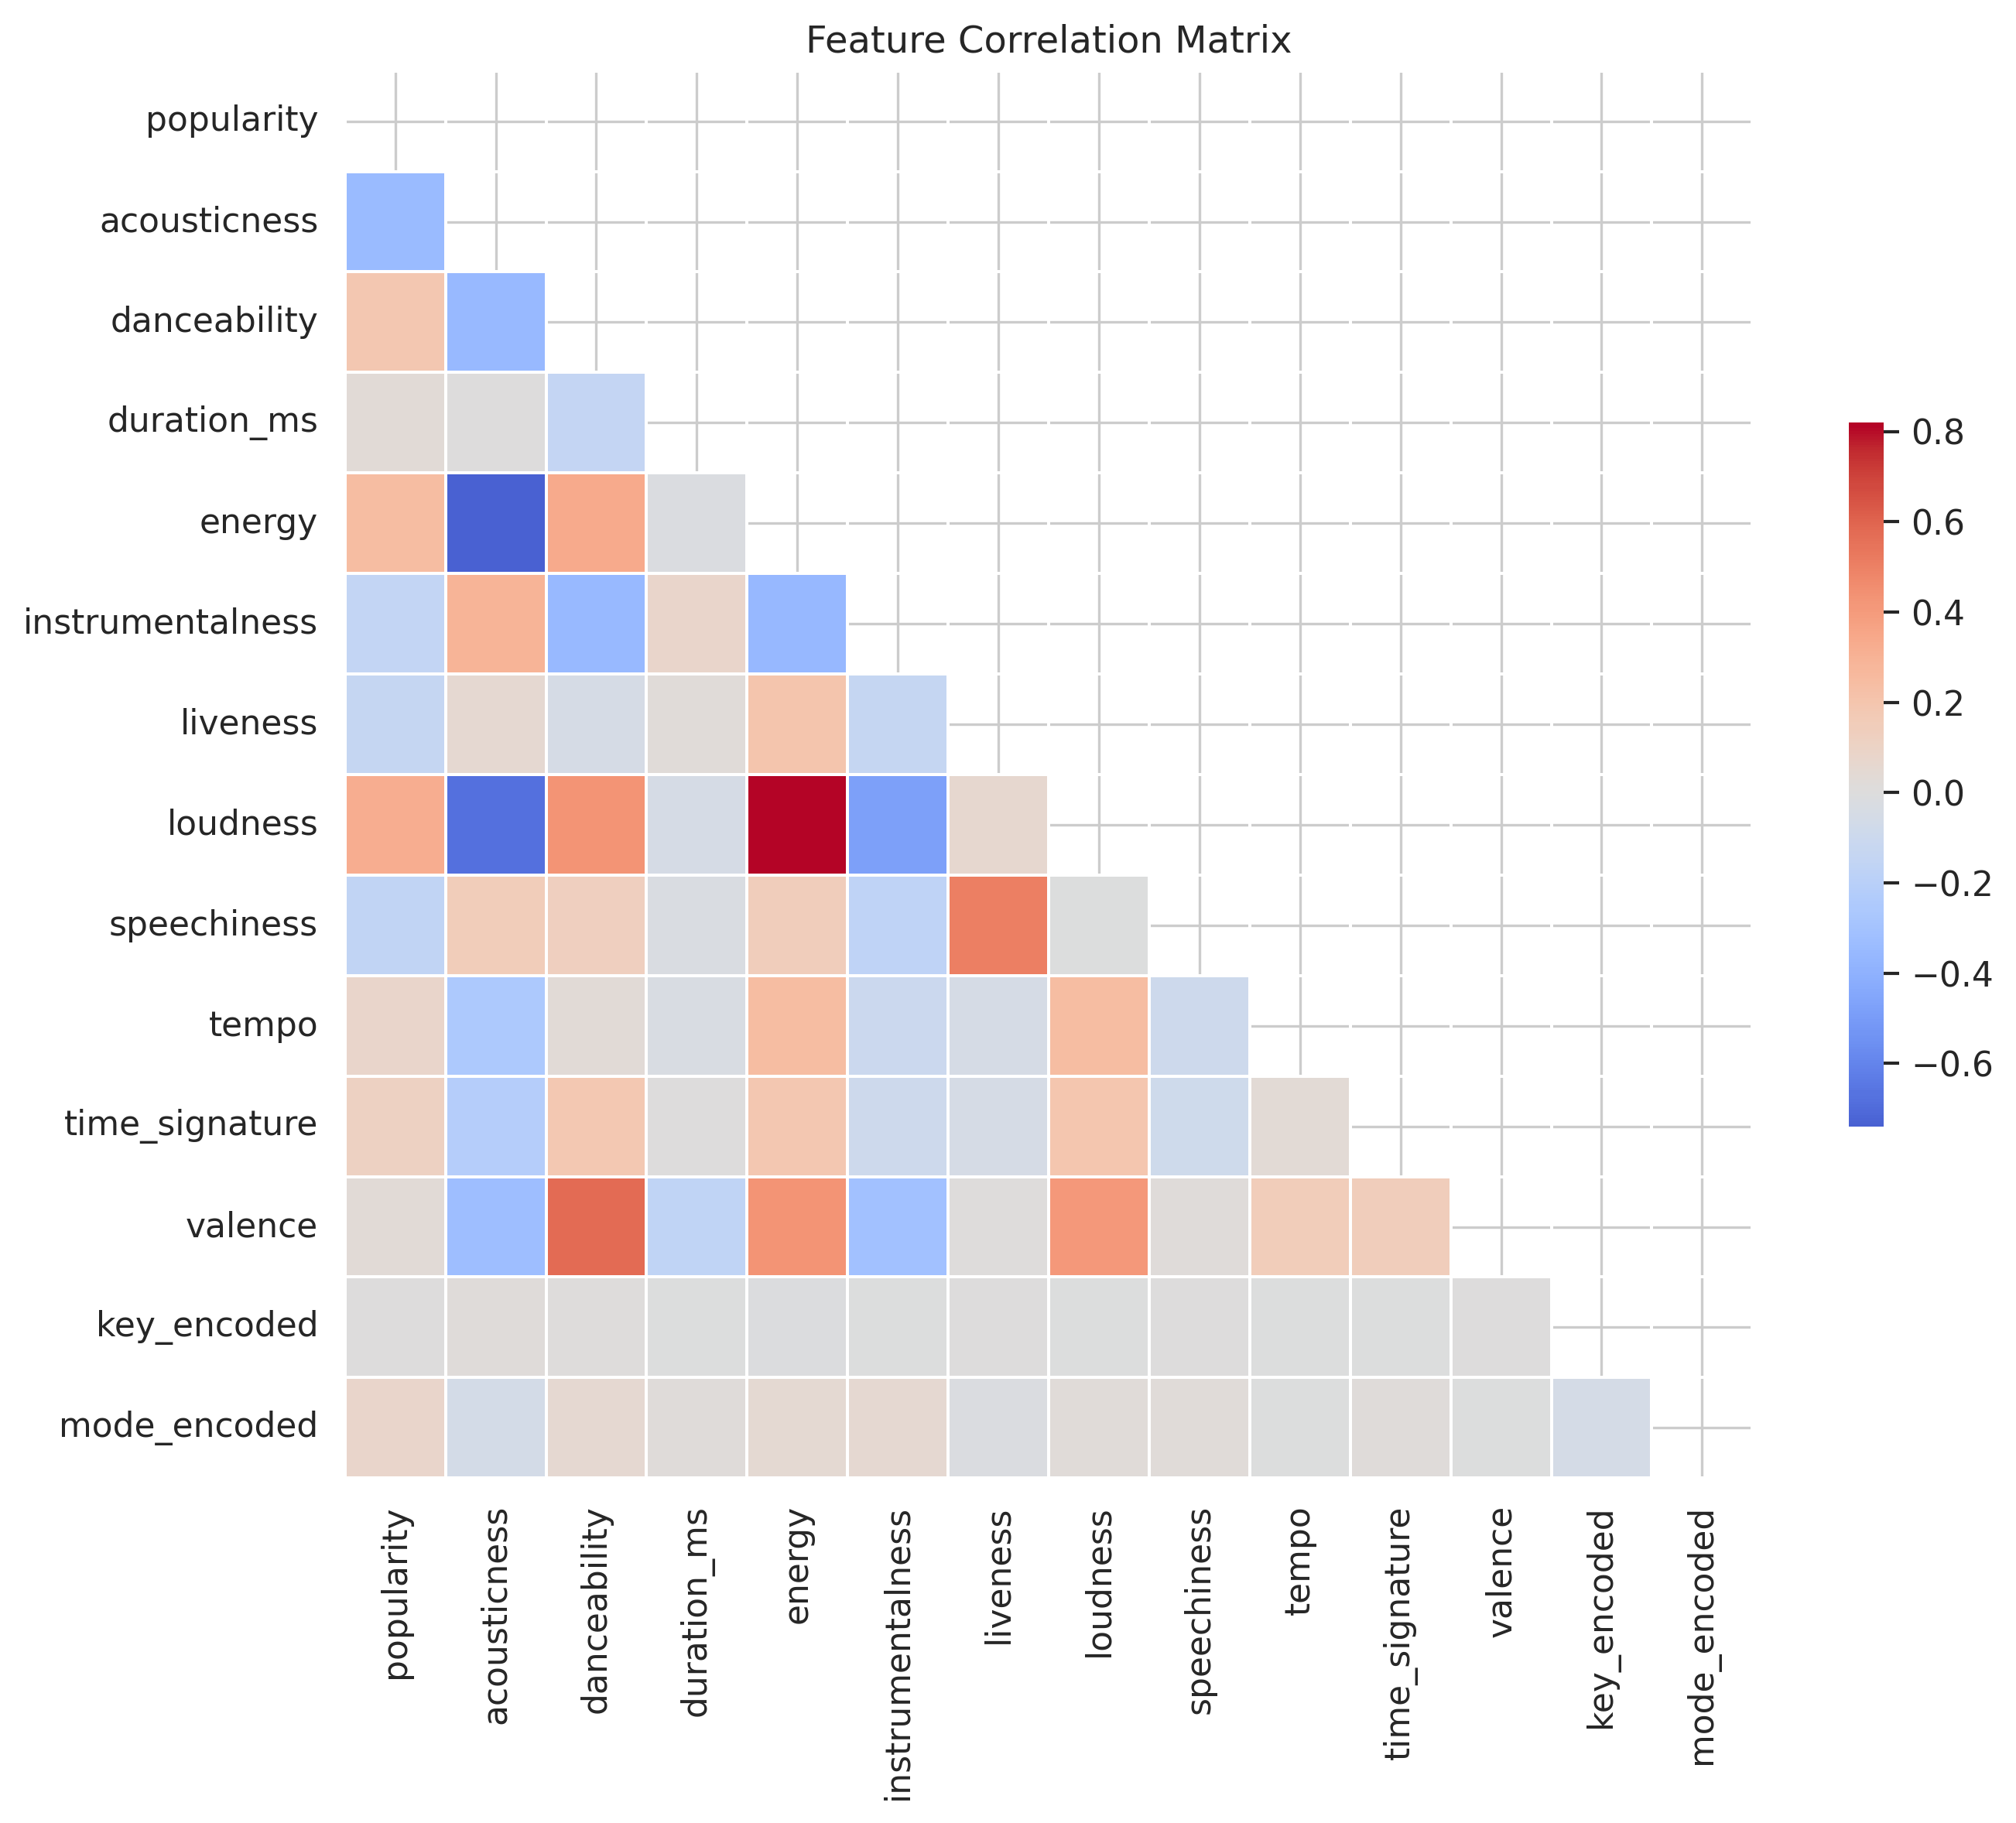
\includegraphics[width=0.7\textwidth]{fig2_correlation.png}
    \caption{Feature Correlation Matrix indicating strong relationships between \texttt{energy}, \texttt{loudness}, and \texttt{acousticness}.}
    \label{fig:corr}
\end{figure}

\subsection{Feature Separability}
Boxplot analysis (Figure \ref{fig:box}) demonstrates that \texttt{acousticness} effectively discriminates Classical music from other genres, while \texttt{energy} separates Electronic music from Classical.

\begin{figure}[H]
    \centering
    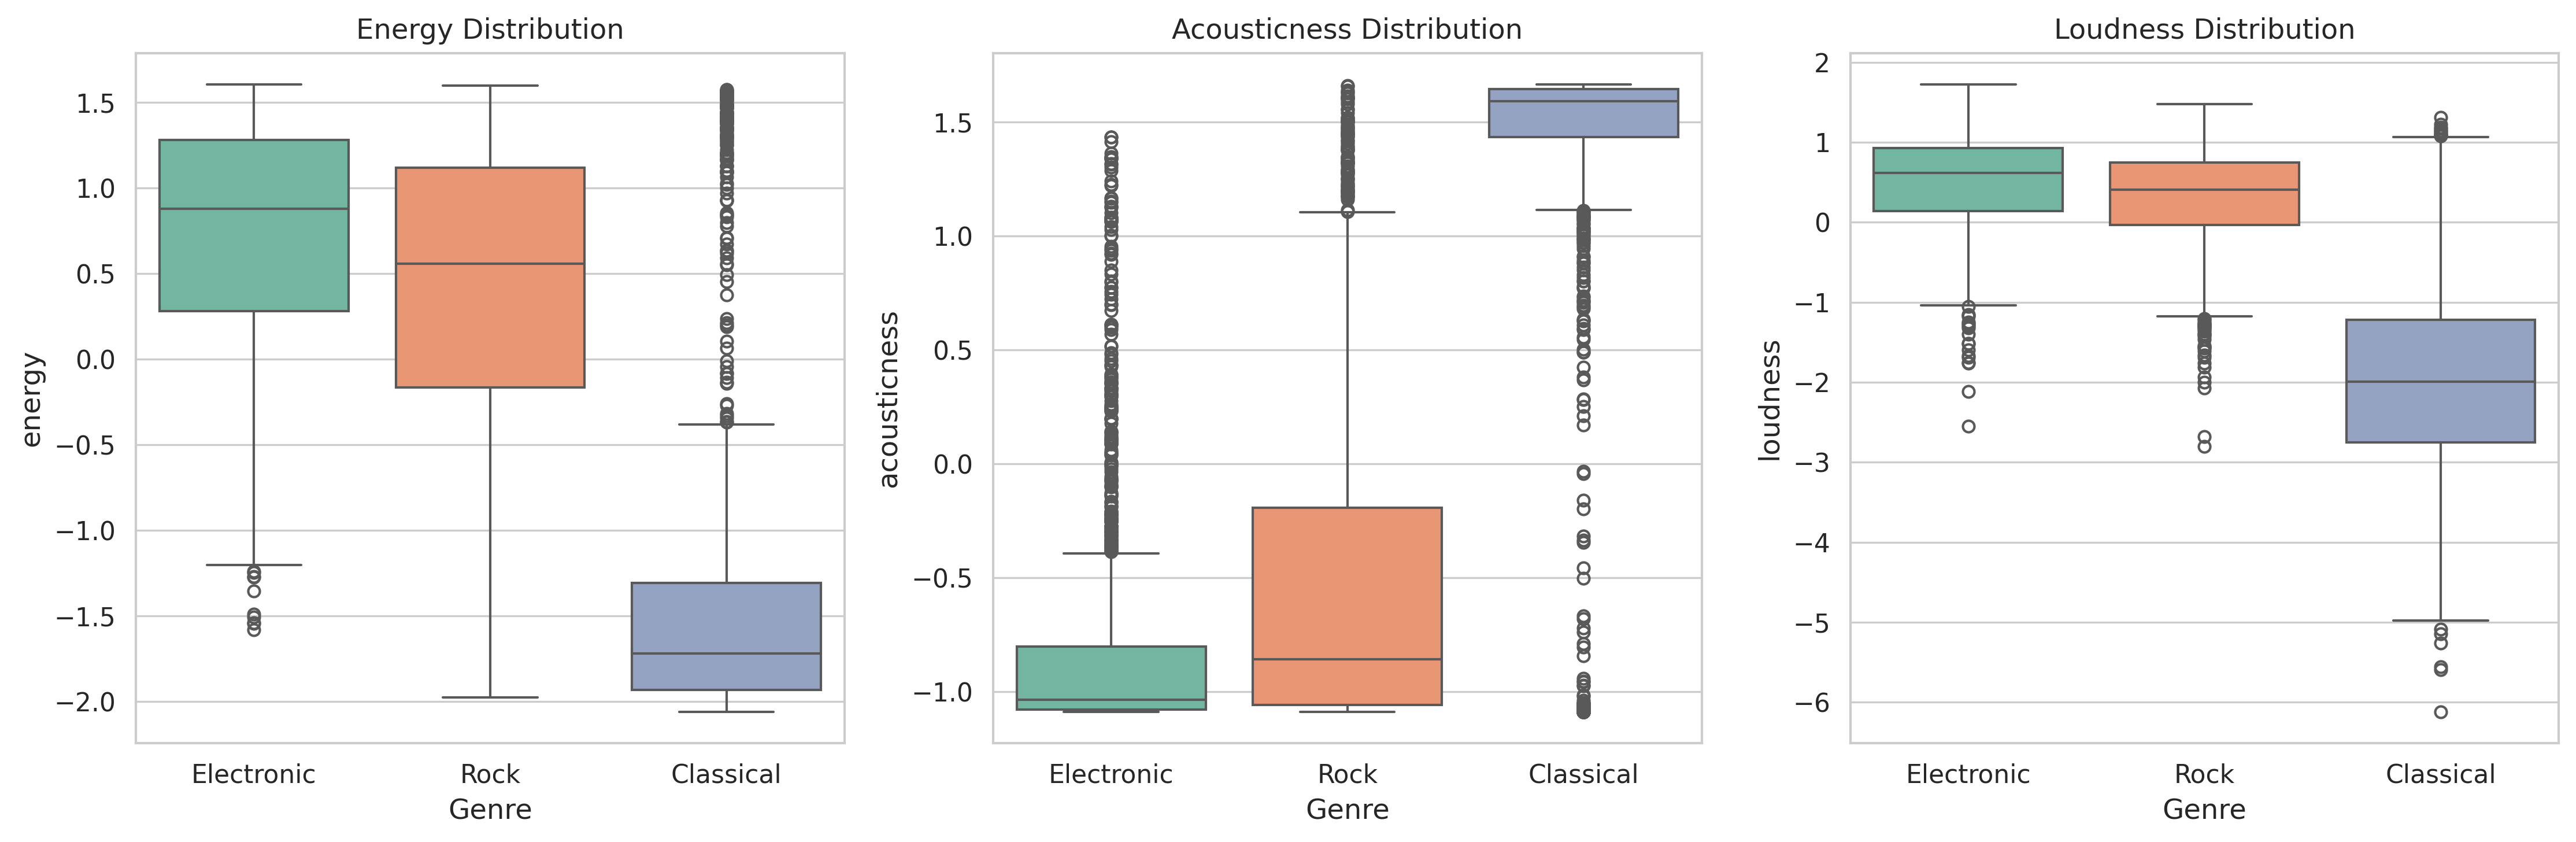
\includegraphics[width=1.0\textwidth]{fig3_boxplots.png}
    \caption{Distribution of key features across three distinct genres.}
    \label{fig:box}
\end{figure}

\section{Modeling Techniques Chosen}
Six modeling techniques were selected to evaluate a range of mathematical approaches to the classification problem.

\subsection{Logistic Regression}
\textbf{Rationale:} Selected as a linear baseline to determine if genre boundaries are linearly separable within the feature space.

\subsection{K-Nearest Neighbors (KNN)}
\textbf{Rationale:} A non-parametric, distance-based approach chosen to exploit potential clustering of genres in the feature space. Hyperparameter tuning indicated that $k=19$ provided the optimal balance between bias and variance (Figure \ref{fig:knn}).

\begin{figure}[H]
    \centering
    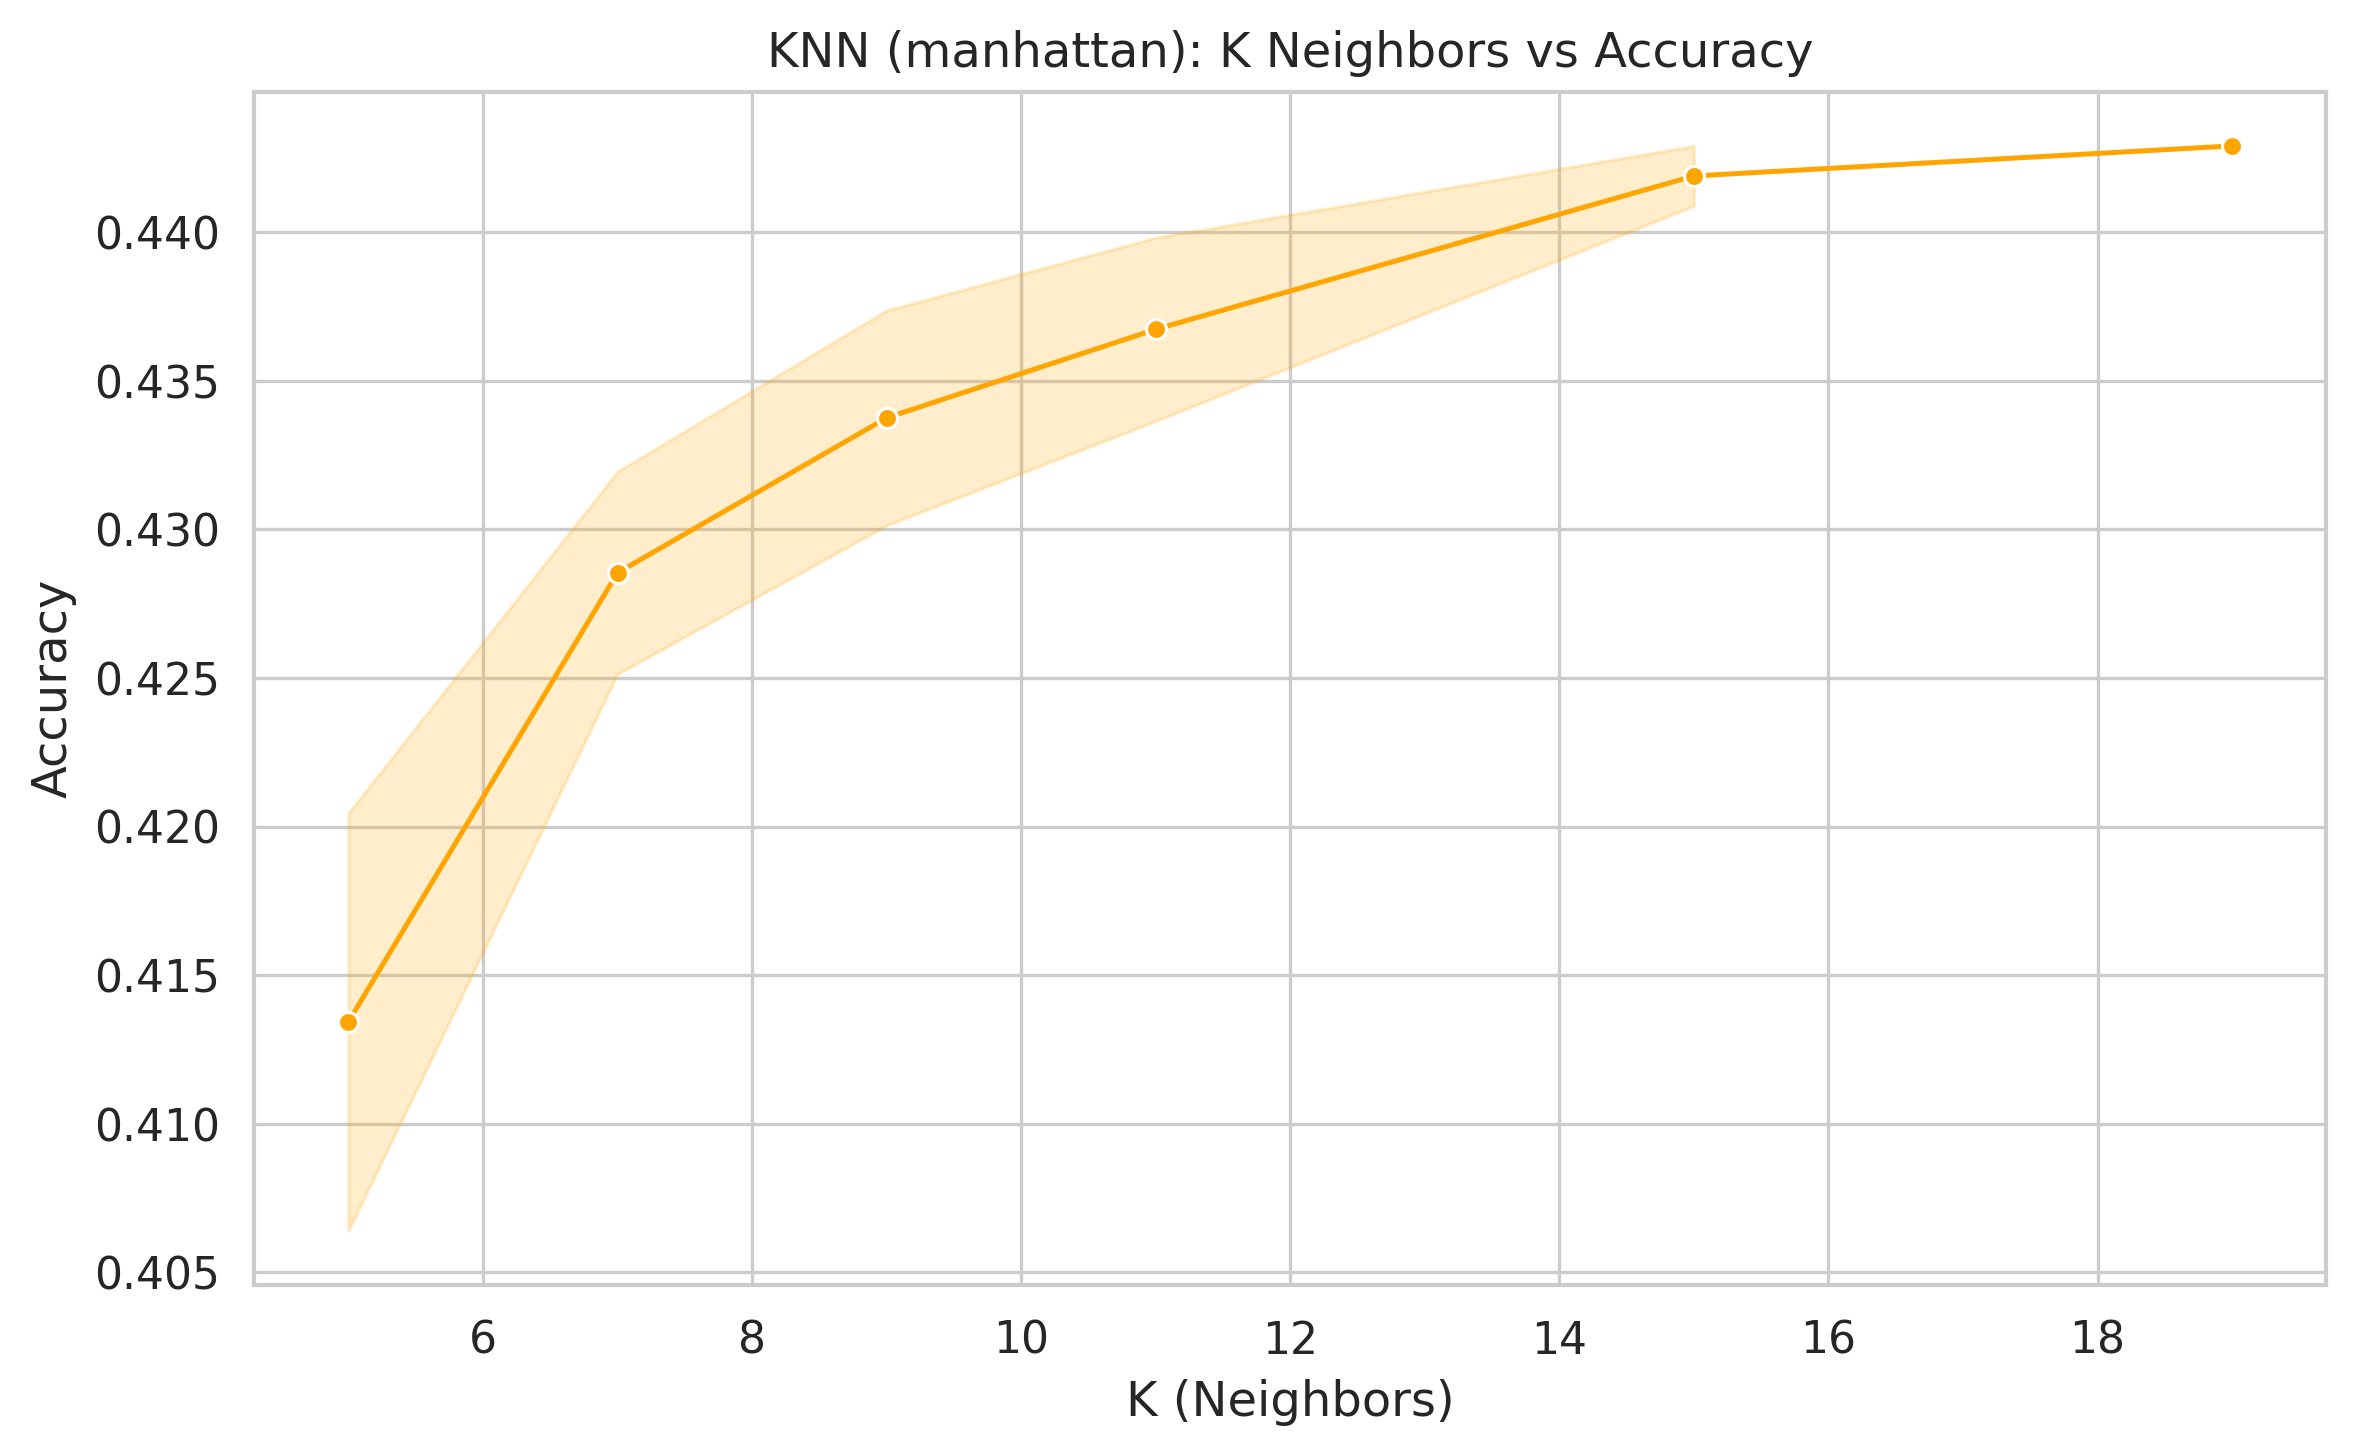
\includegraphics[width=0.6\textwidth]{fig8_knn_k.png}
    \caption{KNN Accuracy vs. Number of Neighbors (k).}
    \label{fig:knn}
\end{figure}

\subsection{Gaussian Naive Bayes}
\textbf{Rationale:} Selected as a probabilistic baseline. While computationally efficient, it assumes feature independence, which serves as a control against the correlated nature of audio data.

\subsection{Random Forest Classifier}
\textbf{Rationale:} An ensemble bagging method chosen for its robustness to noise and ability to model non-linear decision boundaries. Performance plateaued after approximately 300 estimators (Figure \ref{fig:rf}).

\begin{figure}[H]
    \centering
    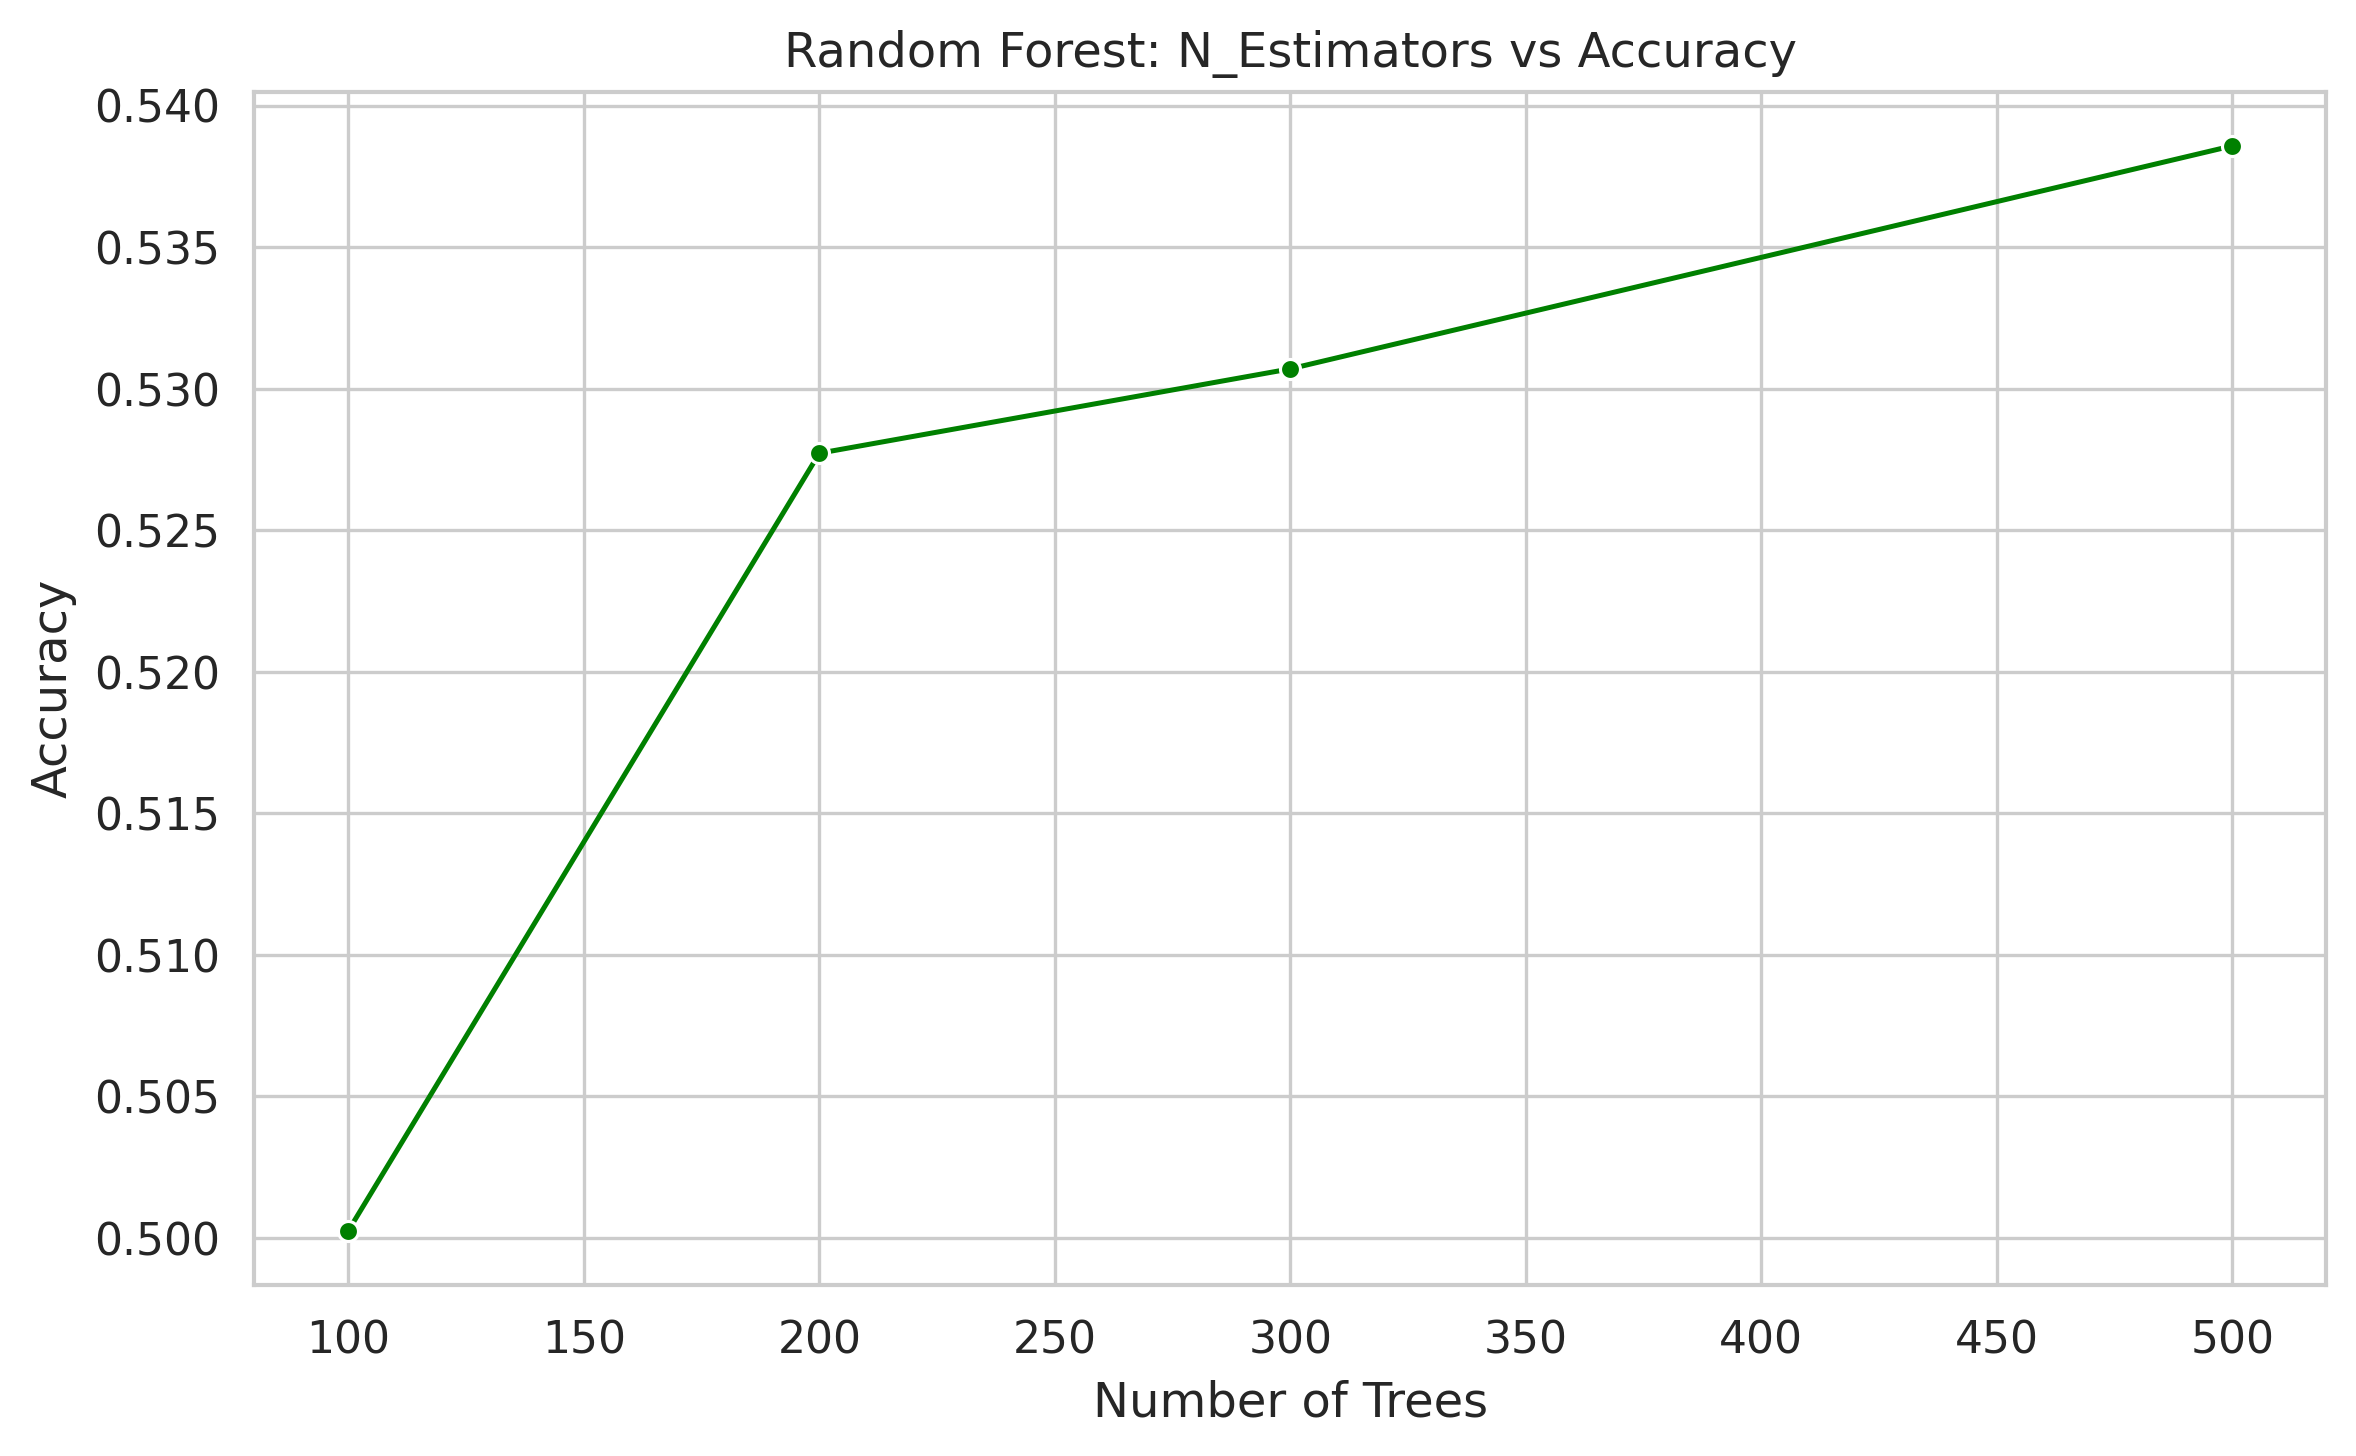
\includegraphics[width=0.6\textwidth]{fig7_rf_estimators.png}
    \caption{Random Forest Accuracy vs. Number of Trees.}
    \label{fig:rf}
\end{figure}

\subsection{XGBoost (Gradient Boosting)}
\textbf{Rationale:} An ensemble boosting method chosen for its state-of-the-art performance on tabular data. Tuning revealed an optimal learning rate of 0.1 (Figure \ref{fig:xgb}).

\begin{figure}[H]
    \centering
    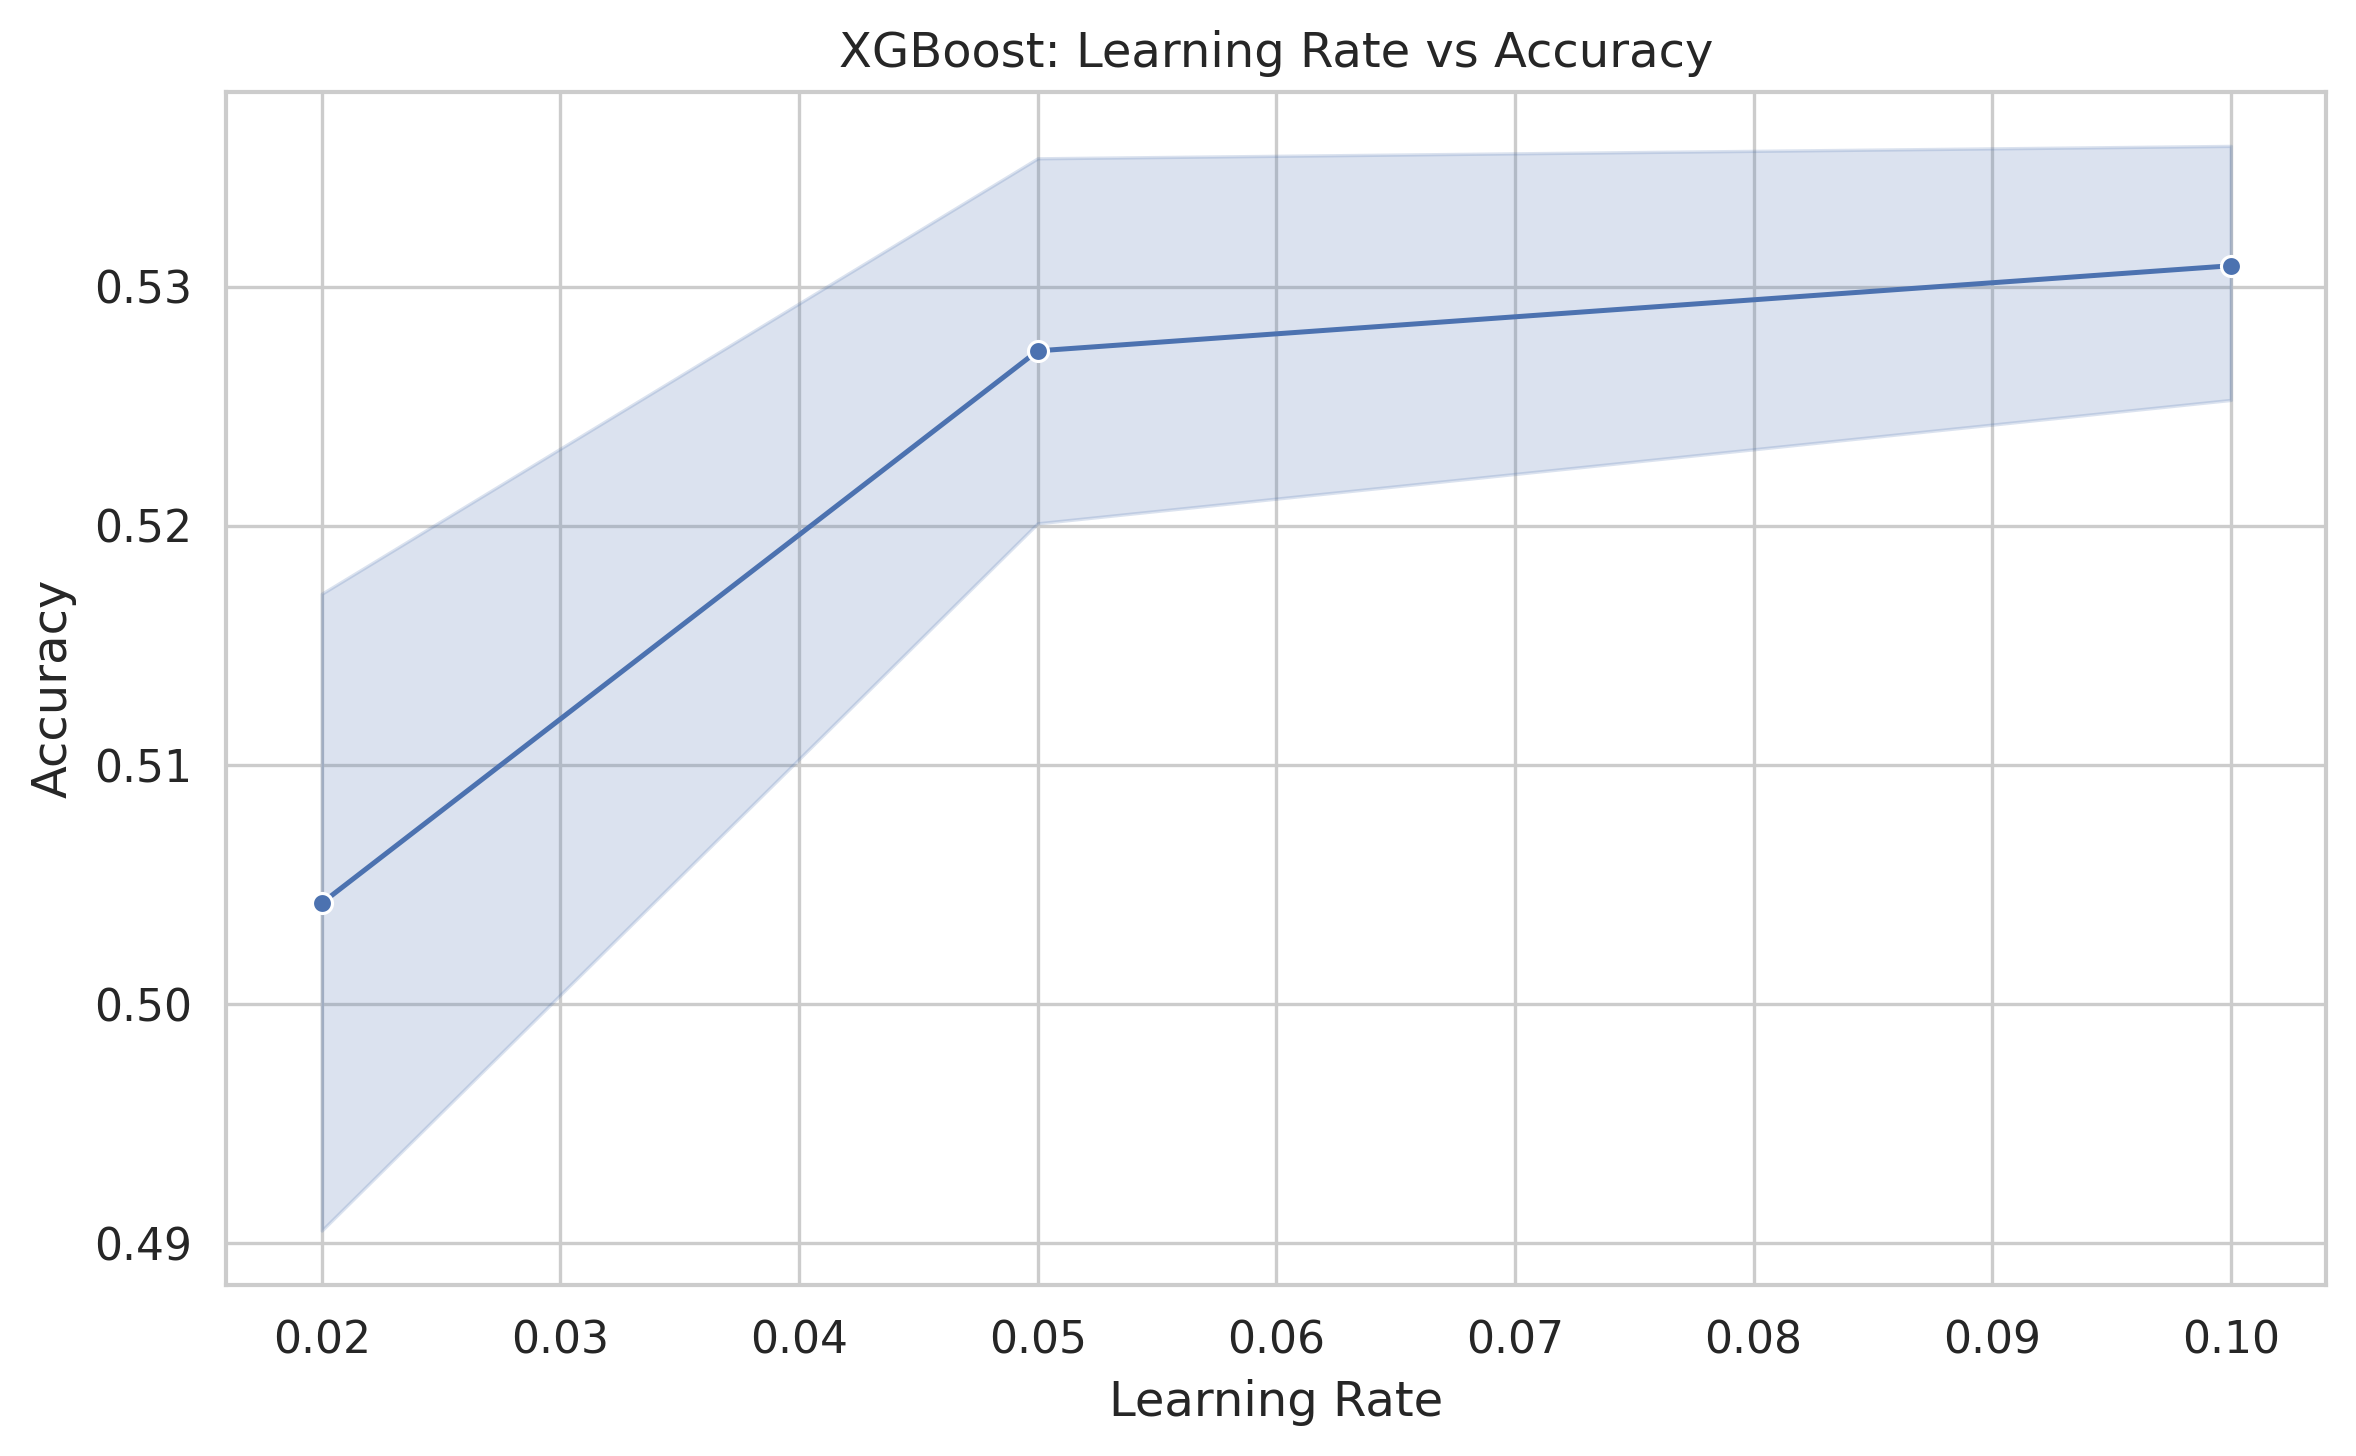
\includegraphics[width=0.6\textwidth]{fig6_xgb_lr.png}
    \caption{XGBoost Accuracy vs. Learning Rate.}
    \label{fig:xgb}
\end{figure}

\subsection{Multilayer Perceptron (MLP)}
\textbf{Rationale:} A deep learning approach using PyTorch, selected to capture complex, high-dimensional feature interactions via a 4-layer architecture.

\section{Reporting of Results}
Model performance was evaluated on the held-out test set ($N=9,397$). Figure \ref{fig:comparison} displays the comparative accuracy of all models.

\begin{figure}[H]
    \centering
    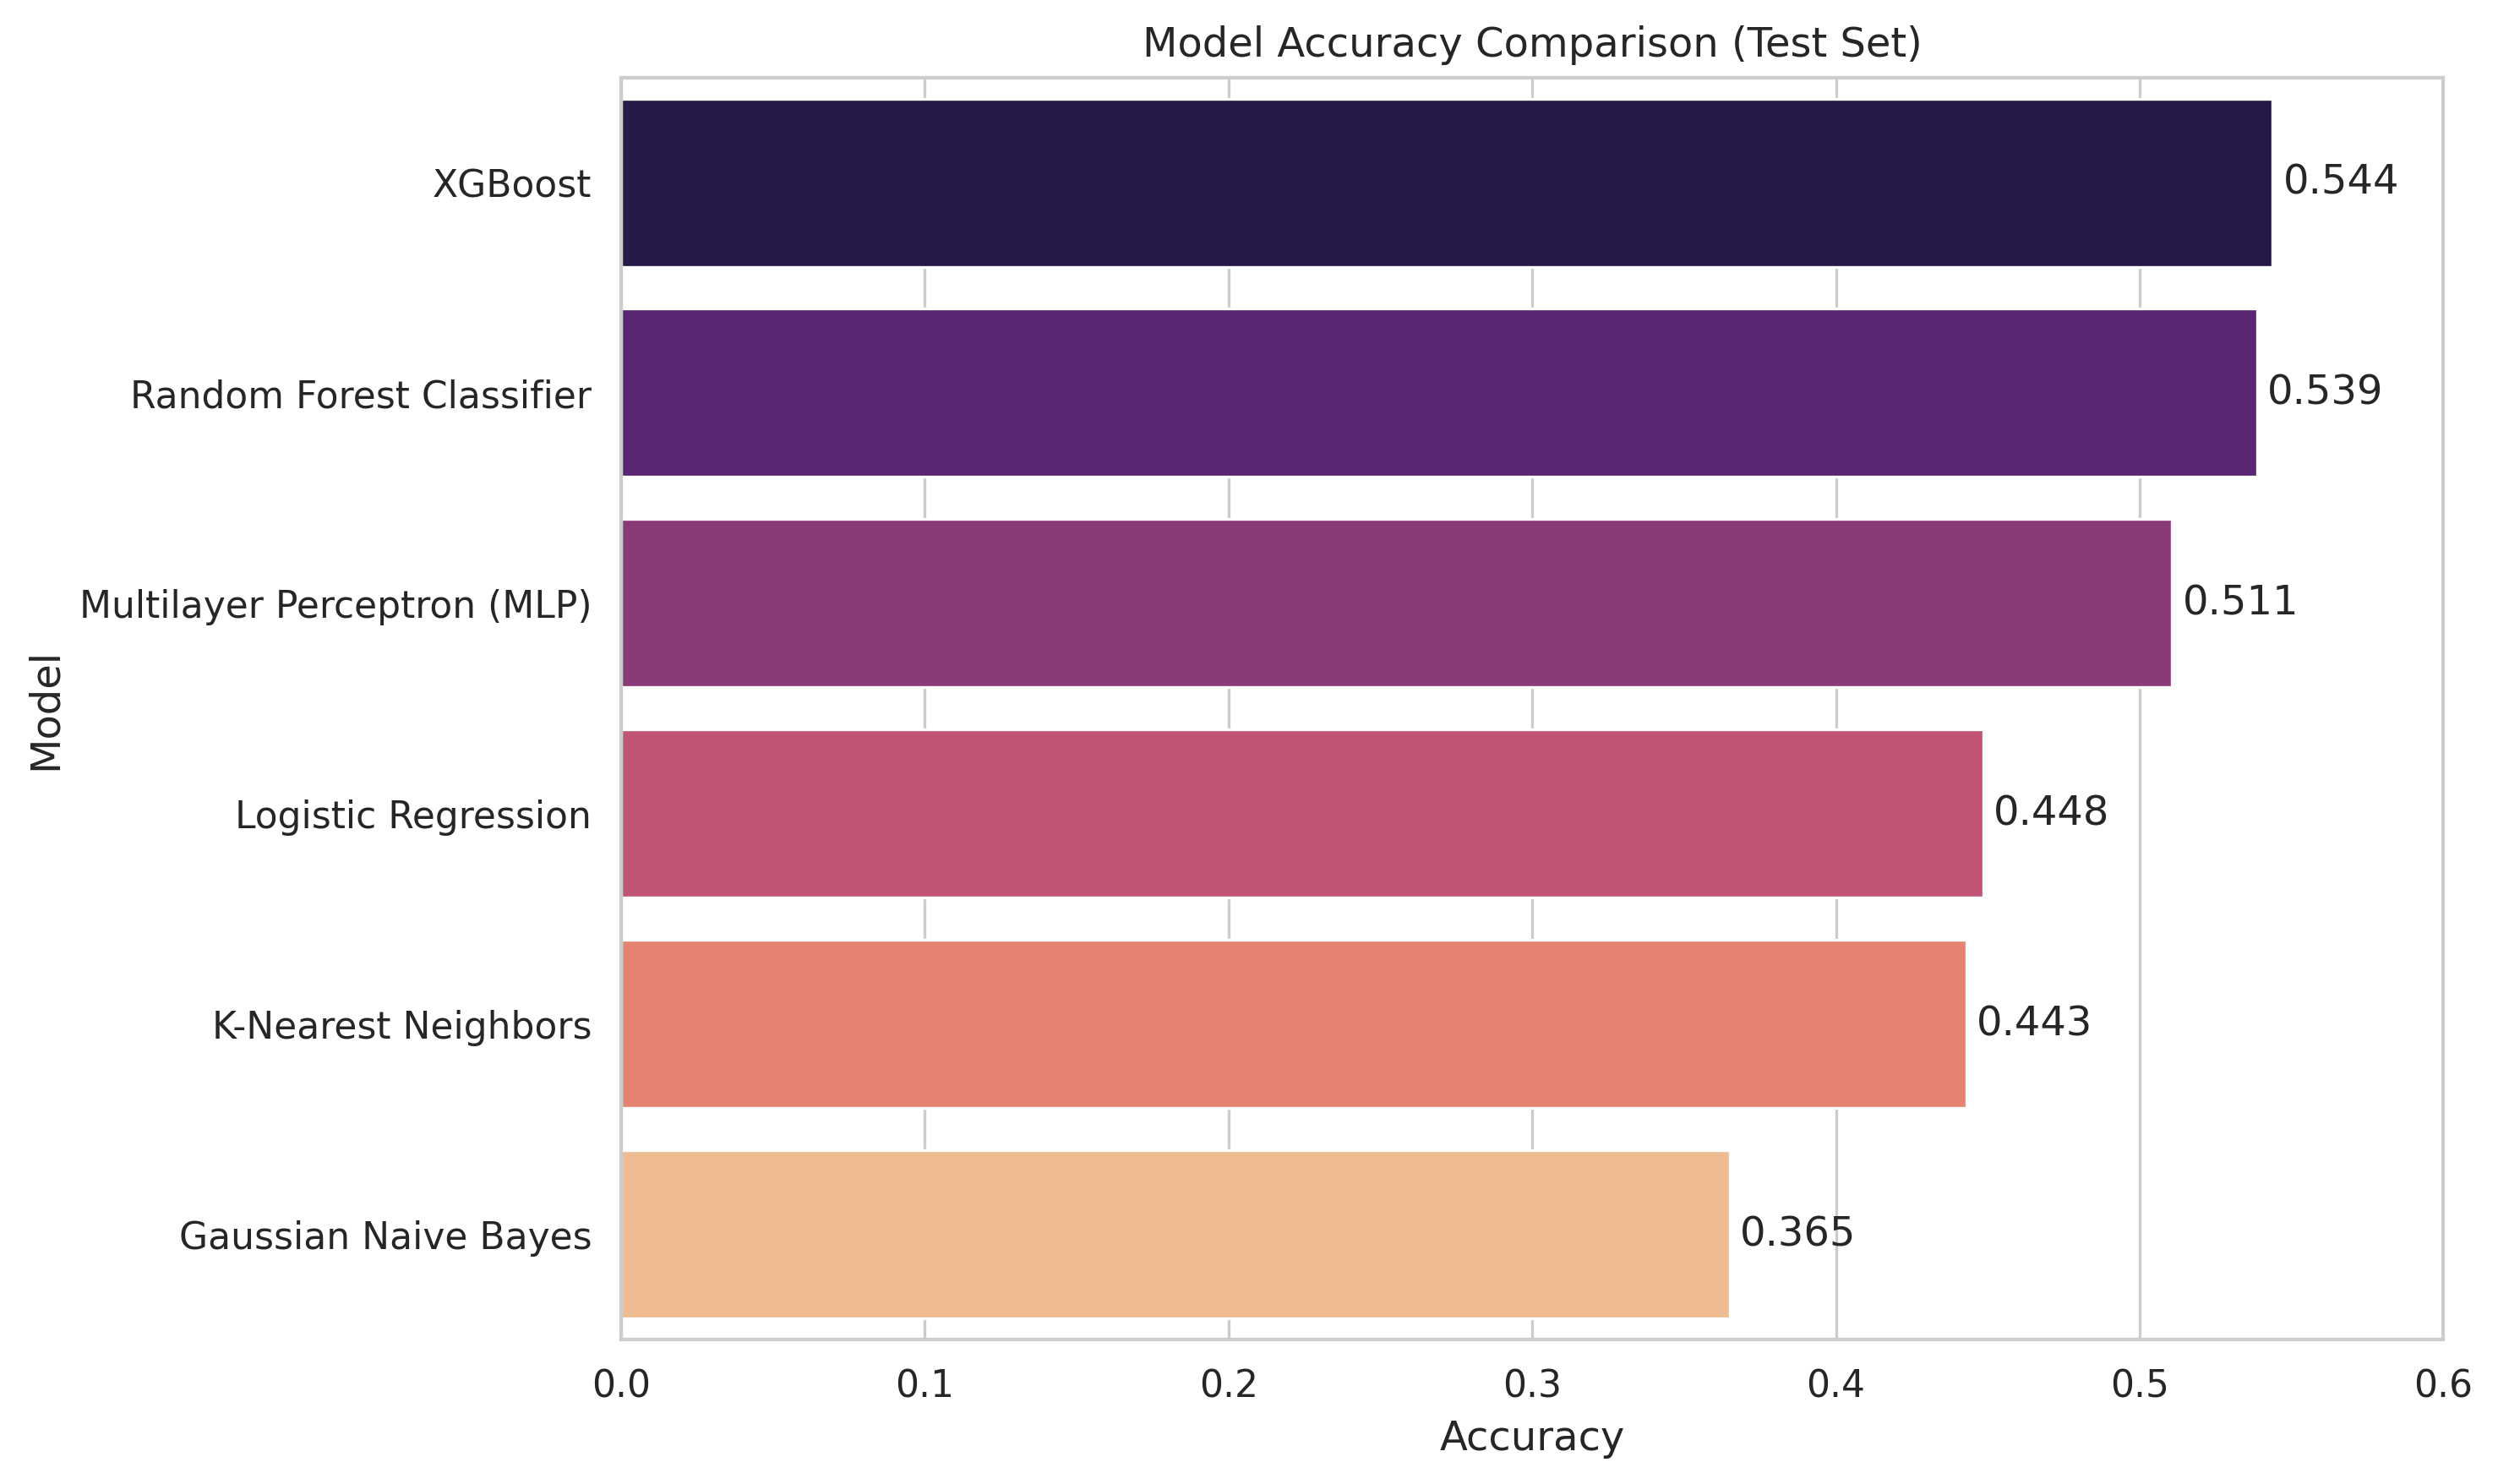
\includegraphics[width=0.8\textwidth]{fig4_model_comparison.png}
    \caption{Comparative accuracy of the six evaluated models.}
    \label{fig:comparison}
\end{figure}

\begin{table}[H]
\centering
\caption{Final Model Leaderboard}
\label{tab:results}
\begin{tabular}{llcc}
\toprule
\textbf{Rank} & \textbf{Model} & \textbf{Accuracy} & \textbf{Weighted F1} \\
\midrule
1 & XGBoost & \textbf{0.5437} & \textbf{0.5400} \\
2 & Random Forest & 0.5386 & 0.5322 \\
3 & MLP (Neural Net) & 0.5107 & 0.5046 \\
4 & Logistic Regression & 0.4484 & 0.4369 \\
5 & KNN & 0.4429 & 0.4402 \\
6 & Gaussian NB & 0.3650 & 0.3405 \\
\bottomrule
\end{tabular}
\end{table}

\section{Interpretation of Results}

\subsection{Predictive Power vs. Random Baseline}
Given 24 distinct classes, a random classifier would achieve an accuracy of approximately 4.1\%. The XGBoost model achieved an accuracy of 54.37\%. This substantial increase over the baseline confirms that the selected audio features contain significant predictive signal regarding musical genre, despite the subjective overlaps between classes.

\subsection{Model Comparison}
\begin{itemize}
    \item \textbf{Tree Ensembles Dominate:} XGBoost and Random Forest outperformed linear and distance-based models by nearly 10\%. This indicates that genre boundaries are highly non-linear and ragged, requiring models that can partition the feature space into complex regions.
    \item \textbf{Neural Networks:} The MLP performed well (51.07\%), surpassing linear models, but did not exceed the performance of tree-based ensembles on this tabular dataset.
    \item \textbf{Linear Limitations:} Logistic Regression (44.84\%) plateaued significantly lower than the top performers, suggesting that the relationships between audio features and genre are not linearly separable.
    \item \textbf{Impact of Correlation:} Gaussian Naive Bayes yielded the lowest accuracy (36.50\%). This confirms the hypothesis derived from the EDA: the strong correlations between features (e.g., \texttt{energy} and \texttt{loudness}) violate the independence assumption of Naive Bayes, degrading its performance.
\end{itemize}

\section{Recommendations of Study}
Based on the analysis, the following recommendations are proposed for future research:

\begin{enumerate}
    \item \textbf{Raw Audio Processing:} To exceed the observed accuracy ceiling of $\approx$55\%, future iterations should incorporate Convolutional Neural Networks (CNNs) applied to Mel-Spectrograms derived from raw audio, rather than relying solely on pre-calculated summary statistics.
    \item \textbf{Hierarchical Classification:} Given the taxonomical nature of music (e.g., "Rock" encompasses "Alternative"), a hierarchical model that predicts the super-genre before refining the specific sub-genre could improve performance.
    \item \textbf{Dimensionality Reduction:} For distance-based models such as KNN, applying Principal Component Analysis (PCA) or manually removing features with low separability (such as \texttt{key} and \texttt{mode}) may reduce noise and improve distance metrics.
\end{enumerate}

\end{document}
